%!TEX root = ../thesis_phd.tex
%%%%%%%%%%%%%%%%%%%%%%%%%%%%%%%%%%%%%%%%%%%%%%%%%%%%%%%%%%%%%%%%%%%%%%%%%%%%%%%%
% cnn.tex:
%%%%%%%%%%%%%%%%%%%%%%%%%%%%%%%%%%%%%%%%%%%%%%%%%%%%%%%%%%%%%%%%%%%%%%%%%%%%%%%%
\chapter{Convolutional Neural Network Event Classifier}
\label{cnn_chapter}
%%%%%%%%%%%%%%%%%%%%%%%%%%%%%%%%%%%%%%%%%%%%%%%%%%%%%%%%%%%%%%%%%%%%%%%%%%%%%%%%

At the core of any particle physics analysis is the selection of signal events,
that is, the events which represent the physical process under study.
Traditionally, features are extracted from event reconstruction and passed
to a machine learning alrorithm, e.g. k-nearest neighbor, neural network, or
decision tree.
While this apporach is generally successful, those classifiers can often
be fooled by reconstruction failures.
Even the most robust reconstruction failures will fall victim to
more pathological event topologies.
Some examples include overlapping particle activity which cannot be resolved
and particles which don't travel far enough to make a recongizable track.

An approach which relies on less reconstruction is thus desirable.
In the case of \nova, this means building a classifier which recieves
the raw detector output as input, so as to cut out the reconstruction as a
middleman.

Since \nova detector output is essentially a pair of images with discrete
pixels, it pays to draw inspiration from the computer vision community.
The recent advances in image classification
\cite{krizhevsky2012imagenet,lecun2015deep,szegedy2014going}
discussed in chapter \ref{nnet_chapter} lend themselves well to the task at
hand.
The implementation discussed in this chapter involves a convolutional neural
network trained on events, treated as images, from \nova simulation and data.
In this approach, the feature extraction units which lead to classification
are trained as convolutional filters in a deep architecture.

\begin{figure}[t]

\begin{subfigure}[c]{\textwidth}
\centering
\begin{subfigure}[c]{0.47\textwidth}
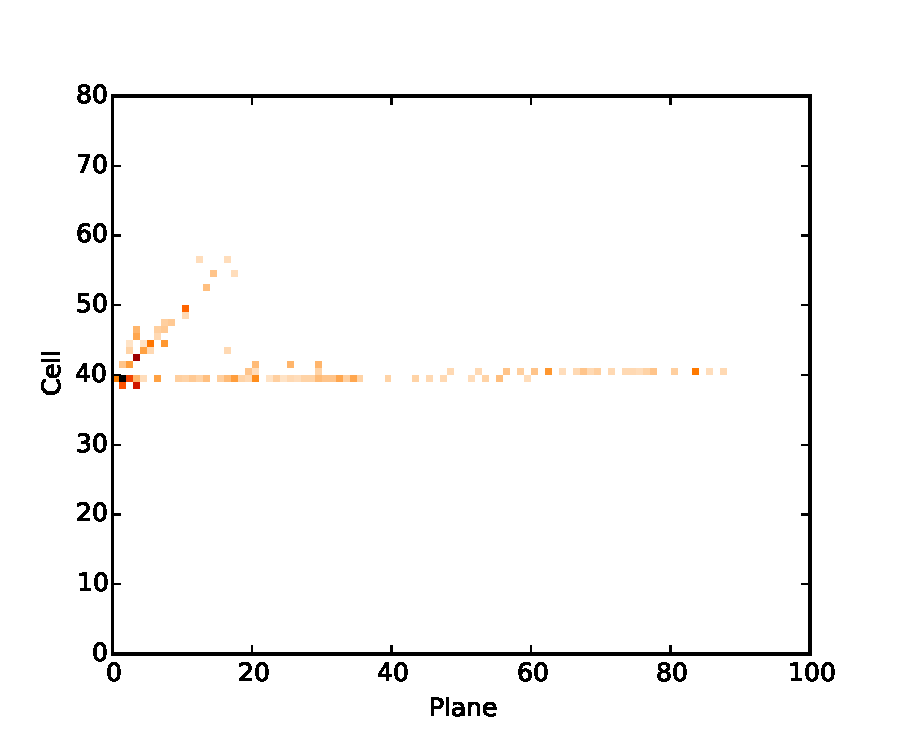
\includegraphics[width=\textwidth]{figures/cnn/view_truetype2_caltype2_event274_x.pdf}
\vspace{-20pt}
\caption*{\xview}
\end{subfigure}
\begin{subfigure}[c]{0.47\textwidth}
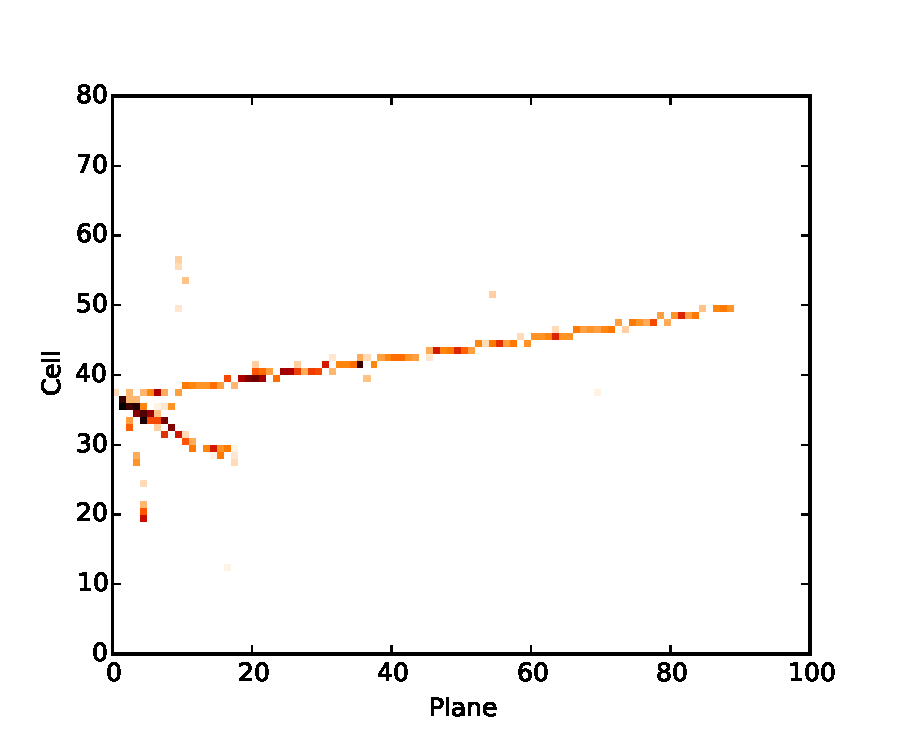
\includegraphics[width=\textwidth]{figures/cnn/view_truetype2_caltype2_event274_y.pdf}
\vspace{-20pt}
\caption*{\yview}
\end{subfigure}
\vspace{-10pt}
\caption{\numu CC interaction.}
\label{pixnumu}
\end{subfigure}

\begin{subfigure}[c]{\textwidth}
\centering
\begin{subfigure}[c]{0.47\textwidth}
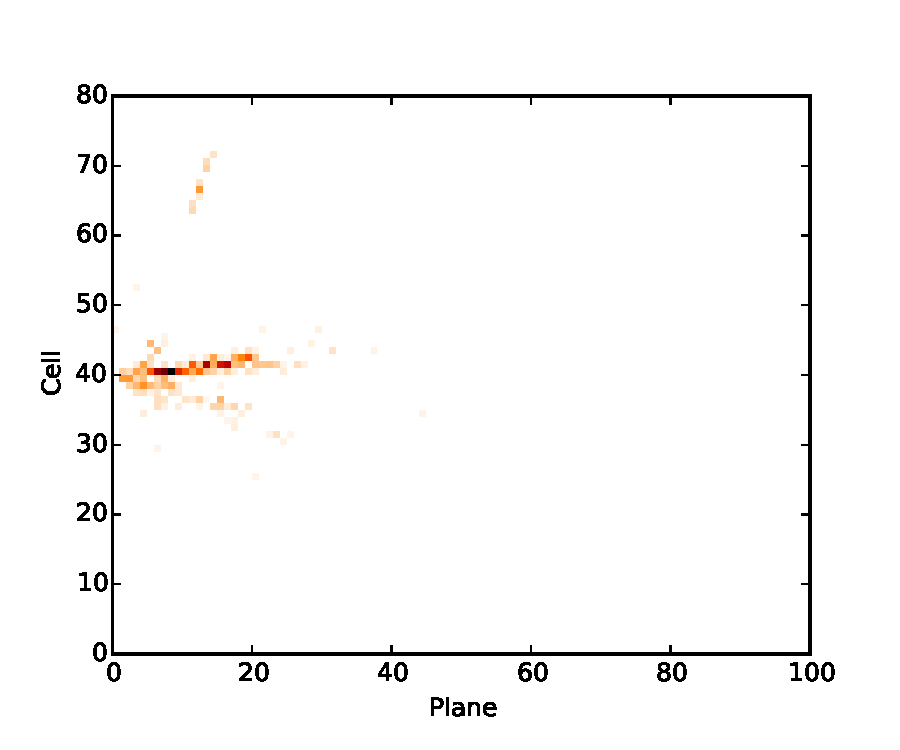
\includegraphics[width=\textwidth]{figures/cnn/view_truetype6_caltype6_event155_x.pdf}
\vspace{-20pt}
\caption*{\xview}
\end{subfigure}
\begin{subfigure}[c]{0.47\textwidth}
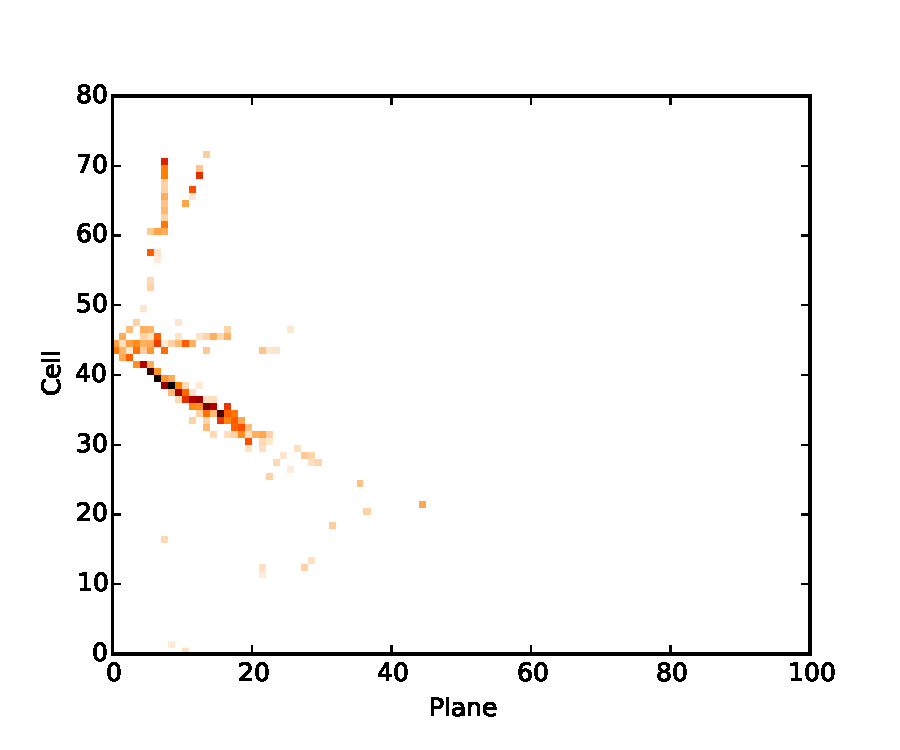
\includegraphics[width=\textwidth]{figures/cnn/view_truetype6_caltype6_event155_y.pdf}
\vspace{-20pt}
\caption*{\yview}
\end{subfigure}
\vspace{-10pt}
\caption{\nue CC interaction.}
\label{pixnue}
\end{subfigure}

\begin{subfigure}[c]{\textwidth}
\centering
\begin{subfigure}[c]{0.47\textwidth}
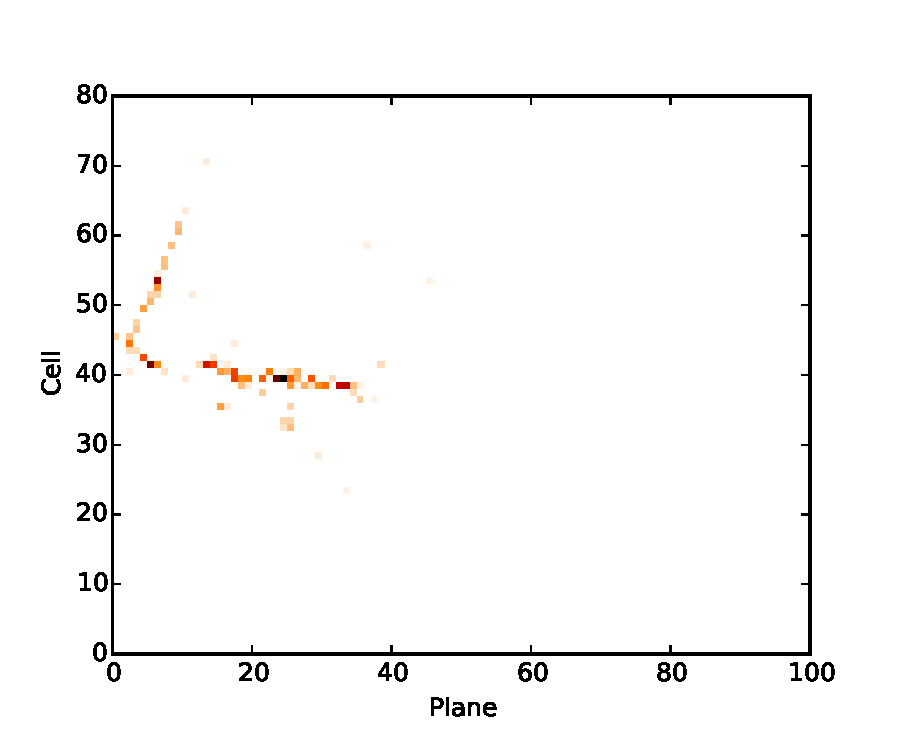
\includegraphics[width=\textwidth]{figures/cnn/view_truetype13_caltype6_event144_x.pdf}
\vspace{-20pt}
\caption*{\xview}
\end{subfigure}
\begin{subfigure}[c]{0.47\textwidth}
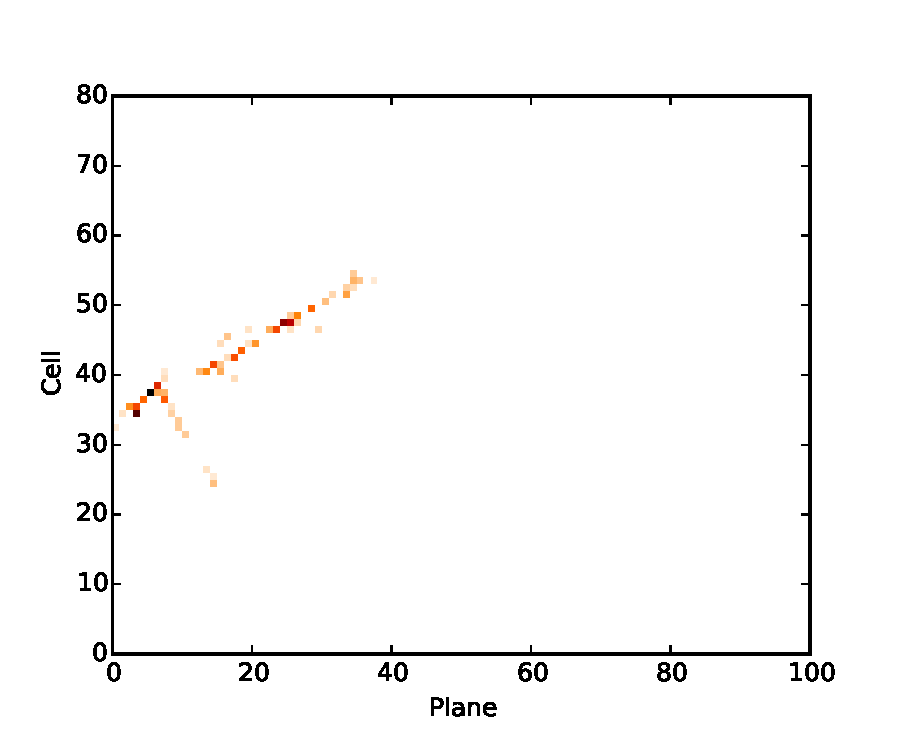
\includegraphics[width=\textwidth]{figures/cnn/view_truetype13_caltype6_event144_y.pdf}
\vspace{-20pt}
\caption*{\yview}
\end{subfigure}
\vspace{-10pt}
\caption{NC interaction.}
\label{pixnc}
\end{subfigure}


\caption{Example images formed from \nova slices.}{
Images such as these are passed as input to the convolutional neural network.
The region of interest is determined by the furthest plane upstream with
activity and the median cell position of all activity
in the 100 plane window spanned by the image.
The pixel intensity is proportional to the calibrated energy deposition
of each cell hit.}
\label{pixelmap}
\end{figure}
\clearpage

\section{\nova Events as Images}

Naively, completely removing reconstruction from the classification pipeline
would mean taking the entire detector readout for a given time window
as input.  The $X$ and $Y$ view could each be treated as an image and passed
to a convolutional neural network.
The neural network, with the positional independence afforded by convolution,
could arguably learn to find neutrino events regardless of where they lie
within the detector.
Sadly, this naive approach falls down for a few reasons.
First, while the ND with roughly 20,000 pixels would produce images of a
manageable scale, the FD with nearly 350,000 pixels is far to large.
Scaling the images down to an acceptable scale would eliminate considerable
detail.
Additionally, calibration of hit energy depositions is not straightforward
when looking at the entire detector.
As discussed in section \ref{calib_atten_section}, calibrated energy deposition
from a hit requires an estimate of distance along the fiber path
between the hit location and readout electronics.
This calibration is important in order to enhance the uniformity of the
event images, leaving behind the effects of attenuation and cell-to-cell
variations would add unnecessary diversity to the training sample.

Rather than using the readout of the entire detector, it is sensible to use
the reconstructed slices discussed in section \ref{slicer_section}.
The performance of DBSCAN in isolating cosmic rays and neutrino interactions
is robust and efficient enough \cite{baird2015thesis} that relying on this
simple reconstruction step will not significantly impact classification
results.
In the case of slices, the distance from the readout electronics is determined
by the mean position of all activity in the opposite view.

Each slice is transformed into an image by locating a region of interest to
capture activity.  The images are 80 cells wide and 100 cells deep in either
view.
The upstream side of the image is the first plane with a hit
in the slice.  In either view, the center of the image is defined by the
median cell position among all hits within the 100 plane window spanned by the
image.
The size and placement of this window ensures that the majority of beam events
are well contained, including \numu CC interactions which are
characteristically extensive as a result of long muon tracks.
Example images can be seen in figure \ref{pixelmap}.

\begin{figure}[t]
\begin{center}

\includegraphics[width=0.7\textwidth]{figures/dummy/dummy.jpg}

\end{center}
\caption{Comparison of continuous hit intensity scale and discretized scale.}{
Data volume is reduced by converting the continuous intensity scale of cell
hit energy depositions into a scale with 256 discrete values.
The discrete scale can be represented with eight bits, offering a significant
savings over a floating point representation.
}
\label{pixelmapadc}
\end{figure}


Pixel intensity is proportional to the calibrated energy deposition
in each cell.
Images are thus interpretable as gray-scale with the shade of
each pixel corresponding to the amount of energy recorded in that cell.
In order to optimize data storage and transfer in the training stage,
the pixel intensities are converted to a scale of 256 discrete values
from the double precision floating point representation calibration result.
This conversion offers a factor of eight savings (eight bit versus 64 bit) in
savings over a floating point representation
without significantly compromising the representational capacity.
The importance of this savings is especially visible in reading data from
disk into memory during training.
A comparison original continuous scale and discrete scale can be seen in figure
\ref{pixelmapadc}.

\begin{figure}[t]
\begin{center}
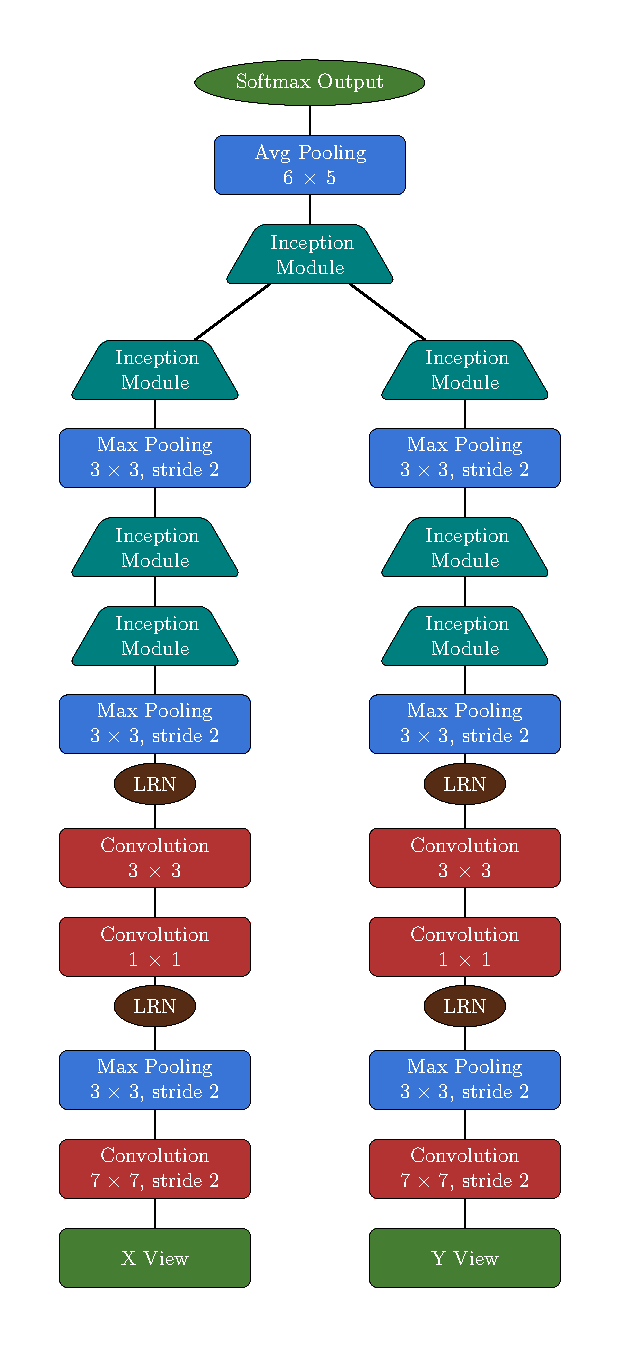
\includegraphics[height=0.9\textheight]{figures/arch/arch.pdf}
\end{center}
\caption{Depiction of the convolutional neural network architecture used
for event classification.}{Starting with the input at the bottom,
the network has separate branches for the \xview and \yview.
Each branch undergoes successive convolution, pooling, and
local response normalization (LRN).  Inception modules are used in downstream layers.
The two views are merged and passed through a final inception module, and
pooled.  The output of the network comes from softmax units.
}
\label{arch}
\end{figure}


\section{Architecture}

The network architecture used in for this analysis is primarily based on
the \googlenet architecture \cite{szegedy2014going} introduced in section
\ref{googlenet_section}.
Initial experiments were performed with a full implementation of \googlenet
for each view, with only the final fully-connected layers merged.
It was observed during training, however,
that the classification of the second intermediate
loss unit showed equivalent classification accuracy to the final loss unit.
The architecture was then pruned and restructured in order to reduce
the total number of operations, and thus the amount of computation required
for training and evaluation.
No degradation was observed in the classification results with the pruned
architecture.
A depiction of the architecture can be seen in figure \ref{arch}.

Input from the \xview and \yview is handled separately in two branches of the
network which are only merged in the final few layers.
Early in the network, images are subjected to $7\times7$ convolution and
$3\times3$ pooling, both with a stride of two.
Using stride two in these early layers scales the images down by a factor of
four.
Local response normalization (LRN) \cite{krizhevsky2012imagenet} is used
to smooth the filtered images.  Two more convolution operations, $1\times1$
and $3\times3$ are used, then another pass of smoothing with LRN, and
$3\times3$ pooling with stride two.  The $1\times1$ convolution serves
as dimensionality reduction in the number of filters.
A pair of inception modules is then used, then another $3\times3$ pooling layer
with stride two and another inception module.  The filter outputs for each view
are then concatenated and passed through another inception module.  A final
pass of average pooling is employed before a softmax layer, which serves as
the output of the network.


In the interest of time, the architecture presented here has only been coarsely
optimized, leaving plenty of room for further study.
It seems quite likely that a significantly more compact network could perform
equally as well.
Classification results could also perhaps be improved through fine tuning of
the architecture.
Eliminating the aggressive downsampling with stride two in the early layers
could significantly increase the level of detail which is available in the
inception modules.
Merging views earlier in the architecture could provide higher levels of
abstraction and greatly reduce the number of operations required.
The effect of LRN should be studied by removing those layers and
comparing results.

\clearpage

\section{Regularization}

A few regularization techniques were applied in order to enhance the ability
of the network to generalize beyond the training sample.
To keep the network weights small, weight decay term was included in the loss
function equal to $2\times 10^{-4}$ times the squared \textit{L2} norm of the
weight vector.
The softmax output layer was also subjected to dropout
\cite{hinton2014dropout}, described in section \ref{regularization_section},
with a probability of 0.4.

Perhaps the most robust defense against over training is more training
data.
In the absence of infinitely large and variegated training samples, however,
we can augment our sample by deliberately randomly changing the input image.
Two techniques were employed in order to add variation to the dataset.
First, Gaussian noise was applied to all pixel intensities with
a standard deviation of 1\%.
Since no Monte Carlo simulation is perfect, adding noise has the added benefit
of training the network to rely less heavily on the simulated intensity
in each pixel.
Second, events were randomly selected to be reflected in the cell dimension,
which is roughly transvese to the beam direction.
Symmetry about in the cell dimension is not perfect; the beam axis is directed
$3^{\circ}$ above detector horizon and attenuation in the optical fiber
causes thresholding to become more significant for hits further from
the readout electronics.
These effects are small, however, and their presence in fact aids in
enhancing variation of the training sample and deweighting precise details
of the Monte Carlo simulation.


\section{Training}

Training was performed using the Caffe framework \cite{jia2014caffe}
using NVIDIA Tesla K20 and K40 graphics processing units (GPU).
Weight updates were
performed using the basic stochastic gradient descent (SGD)
\cite{reed1999neural} procedure described in chapter \ref{nnet_chapter}.

The first training set consisted of ... gotta go on

Due to GPU memory constraints, a mini-batch training scheme was employed.
In mini-batch training, gradients used in weight updates are averaged over
small sub-samples of the training dataset rather than the entire sample.
After calculating the gradient for a batch, it is flushed from memory
and the next batch is loaded.
Batches are reused after each full pass over the training dataset
A batch size of 32 was used to train the network.
Each pass over a mini-batch is referred to as an \textit{iteration};
a full pass over the dataset is called an \textit{epoch}.

The initial learning rate was set to 0.01.
During the training, the learning rate was decreased by a factor of 0.96
according to a prescribed schedule.
The learning rate was decreased after the first 100,000 iterations, again
after the next two sets of 50,000 iterations, then again after four sets of
25,000 iterations, and then after each subsequent 10,000
iterations.

After 640,000 iterations, an error was observed in the architecture.
Rather than having the intended 15 nodes in the softmax output layer,
the architecture had accidentally been configured with 1,000 nodes in that
layer.
The architecture was modified to have the correct number of nodes, and training
was resumed by reloading trained weights from all layers but the output.
Upon resuming training, the learning rate was set to 0.002, roughly equal to
the learning rate reached after 640,000 iterations.
The decrease schedule, however, was started from the beginning rather
than reverting to the once every 10,000 iteration schedule
that would have been employed beyond iteration 640,000.

After 970,000 total iterations, XXXXX events from cosmic ray data were added
to the training example.



%%%%%%%%%%%%%%%%%%%%%%%%%%%%%%%%%%%%%%%%%%%%%%%%%%%%%%%%%%%%%%%%%%%%%%%%%%%%%%%%
